\documentclass{controle}
\usepackage{main}

\title{Contrôle n°3 : Fonctions inverses; suites géométriques}
\date{9 Janvier 2026}
\author{TSTMG1}

\begin{document}
\maketitle

\instructions[Autorisée]

\begin{questions}
\titledquestion{Sommes géométrique}[6]
Calculer les sommes géométriques suivantes :
\begin{parts}
\part[2] $1 + 2 + 2^2 + \dots + 2^{10}$
\part[2] $1 + 1,4 + 1,4^2 + \dots + 1,4^{25}$
\part[2] $1 + 0,7 + 0,7^2 + \dots + 0,7^{34}$
\end{parts}
\titledquestion{Fonction inverse}[7]
Soit $f : x \mapsto 4x - 500 + \dfrac{676}{x}$ définie sur $[-20;10]$.
\begin{parts}
\part[1] On admet que $f$ est dérivable sur $[-20;10]$. Montrer que pour tout $x$ dans $[-20;20]$,
\begin{equation*}
f'(x)= 4 - \dfrac{676}{x^2}
\end{equation*}
\part[2] En déduire que pour tout $x$ dans $[-20;10]$,
\begin{equation*}
f'(x) = \dfrac{4(x-13)(x + 13)}{x^2}
\end{equation*}
\part[2] Compléter le tableau de signes de $f'$ et le tableau de variations de $f$ :
\begin{center}
\begin{tikzpicture}
\tkzTabInit{$x$/1, Signe de $x-13$/1, Signe de $x + 13$/1, Signe de $f'$/2, Variations de $f$/2}{$-20$,,,$10$};
\end{tikzpicture}
\end{center}
\part[2] En déduire le minimum de la fonction, et pour quel $x$ ce minimum est atteint.
\end{parts}
\titledquestion{Suite arithmético-géométrique}[7]
Soit $(u_n)_{n \in \N}$ la suite définie par la relation de recurrence suivante :
\begin{equation*}
\begin{cases}
u_0 &= 4\\
u_{n+1} &= 9u_n + 24
\end{cases}
\end{equation*}
\begin{parts}
\part[0,5] Calculer $u_1$, $u_2$ et $u_3$.
\part[0,5] La suite $(u_n)$ est-elle géométrique ? arithmétique ?
\part[1] Soit $(v_n)$ la suite définie, pour tout $n \in \N$,
\begin{equation*}
v_n = u_n + 3
\end{equation*}
\part[1] Calculer $v_0$.
\part[2] Montrer que la suite $(v_n)$ est géométrique de raison $9$.
\part[0,5] En déduire une la formule explicite de $v_n$ en fonction de $n$.
\part[1] En déduire une expression de $u_n$ en fonction de $n$.
\part[0,5] Calculer $u_{20}$.
\end{parts}
\end{questions}
\end{document}